%%%--------------------------------------------------------------------------------------------
\documentclass[a4paper, man, natbib]{apa6}
\usepackage[english]{babel}
\usepackage[utf8x]{inputenc}
\usepackage{mathtools}
\usepackage{amssymb}
\usepackage{graphicx}
\usepackage[colorinlistoftodos]{todonotes} 
\usepackage{etoolbox}

% \usepackage{lineno}

\title{The Effect of Episodic Retrieval on Inhibition in Task Switching}
\shorttitle{Episodic Retrieval \& Inhibition}
\author{James A. Grange, Agnieszka W. Kowalczyk, and Rory O'Loughlin}
\affiliation{School of Psychology, Keele University, UK}

\note{{\bf Word Count:} 3,857 (Main body \& references, not including abstract.)}
% 577 words in referecnes.
% \note{{\bf Under Review---Please, no direct quotes.}}

% command to insert editing comments or track changes
\newcommand{\jg}[1]{\textcolor{blue}{$^{\textrm{}}${#1}}}

%command for R symbol
\newcommand{\R}{R}

\authornote{Please address correspondence to James A. Grange, School of Psychology, Dorothy Hodgkin Building, Keele University, Keele, UK, ST5 5BG. Email: grange.jim@gmail.com. All raw data and analysis code are available to download at http://bit.ly/1OgH9v0.}

\leftheader{Grange, Kowalczyk, \& O'Loughlin}


\abstract{Inhibition in task switching is inferred from n--2 repetition costs: the observation that AB$A$ task switching sequences are responded to slower than CB$A$ sequences. This is thought to reflect the persisting inhibition of task A, which slows re-activation attempts. \cite{Mayr2002} reported an experiment testing a critical non-inhibitory account of this effect, namely episodic retrieval: If the trial parameters for task A match across an ABA sequence, responses should be facilitated due to priming from episodic retrieval; a cost would occur if trial parameters mismatch. In a rule-switching paradigm, Mayr reported no significant difference in n--2 repetition cost when the trial parameters repeated or switched across an ABA sequence, in contrast to the episodic retrieval account. This conclusion rests on accepting a null hypothesis, which cannot be achieved with null hypothesis significance testing. Here we provide a replication of the critical aspects of Mayr's design. Using Bayesian analysis to quantify evidence for or against a null hypothesis, we find evidence for reduced n--2 repetition costs when trial parameters repeat compared to when they switch. In contrast to Mayr's conclusion, we suggest that episodic retrieval can influence the measure of inhibition in task switching, although it cannot explain it entirely.}

\keywords{Task switching; inhibition, episodic retrieval, cognitive control}

\begin{document}
\maketitle

%----------------------
Stimuli in the human environment typically afford more than one action. Sat at a computer, for example, there are many tasks that could be performed, such as writing a manuscript, checking the weather, or playing a game of online chess. In order to act in a goal-directed manner, humans must be able to \emph{select} the relevant task (writing a paper) in the face of competing tasks (playing chess), and maintain this task in an active state so that it can be performed. However, such \emph{stable} task representations must also be \emph{flexible}, so that they can be removed when the goals change (such as when the phone rings). This tension between the need for stability and flexibility of task representations has been called the \emph{stability--flexibility dilemma} \citep{Goschke2000}. 

How the cognitive system solves the stability--flexibility dilemma has been studied using the task switching paradigm \citep{Grange2014a,Kiesel2010,Vandierendonck2010}, wherein participants have to make speeded responses to simple cognitive tasks. For example, participants might be presented with number stimuli, and be asked to switch between judging whether the stimulus is odd/even or lower/higher than five. One cognitive process thought to be essential for task switching performance is the inhibition of competing tasks. Evidence for inhibition comes from the backward inhibition paradigm \citep{Koch2010, Mayr2000}, where participants are required to switch between three tasks (A, B, and C).  It is a consistent finding that AB$A$ task switching sequences are performed slower and with less accuracy than CB$A$ sequences. This \emph{n--2 task repetition cost} is thought to reflect the persisting inhibition of task A in an ABA sequence, which hinders its re-activation in the last trial of the triplet.

The n--2 task repetition cost is important as it appears to be robust against non-inhibitory explanations \citep{Mayr2007}. One potential explanation of the n--2 task repetition cost that does not assume inhibition was explored by \cite{Mayr2002}. This \emph{episodic retrieval} account \citep{Neill1997} suggests (adapted to a task switching context) that when a task has been performed an episodic trace of trial parameters (such as the cue, stimulus characteristics, and the response made) is stored in memory. When this task is cued again, retrieval of the most recent episodic trace occurs. If the parameters of the presented trial differ from that of the retrieved episode (e.g., a different response is required), a mismatch cost occurs relative to if the retrieved episode matches parameters of the current trial (which will prime performance). Thus, according to this account, n--2 task repetition costs reflect a mismatch cost, as trial parameters typically differ between both instances of task A in an ABA sequence.

\cite{Mayr2002} assessed this alternative explanation by developing a paradigm where the match between trial parameters across an ABA sequence could be manipulated (see Figure \ref{fig:mayrExperiment}). Participants were required to apply a spatial transformation of a target's location according to one of three stimulus--response rules (vertical, horizontal, or diagonal transformations). For example, if the target is in the bottom-left of the display and the current rule is ``vertical'', the correct response would be an upper-left response (as this reflects a vertical transformation of a bottom-left target). The parameters that might be stored in an episodic trace include (at least) the cue presented, the target's location, and the response made. In this paradigm, trial parameters can either match or mismatch across ABA and CBA sequences\footnote{Note that with one cue per task, the cue for task A will always be the same across an ABA sequence.}. For example, if the target is in the same location for task A across an ABA sequence, the same response will be required (i.e., an n--2 response repetition). In this case, the episodic retrieval account would predict facilitated performance relative to an n--2 response switch as in the former case the current trial parameters match perfectly the retrieved episodic trace. Thus, the episodic account would predict reduced n--2 task repetition costs for n--2 response repetitions compared to n--2 response switches (where there is a mismatch between trial parameters and the retrieved episodic trace).

\begin{figure}
\begin{center}
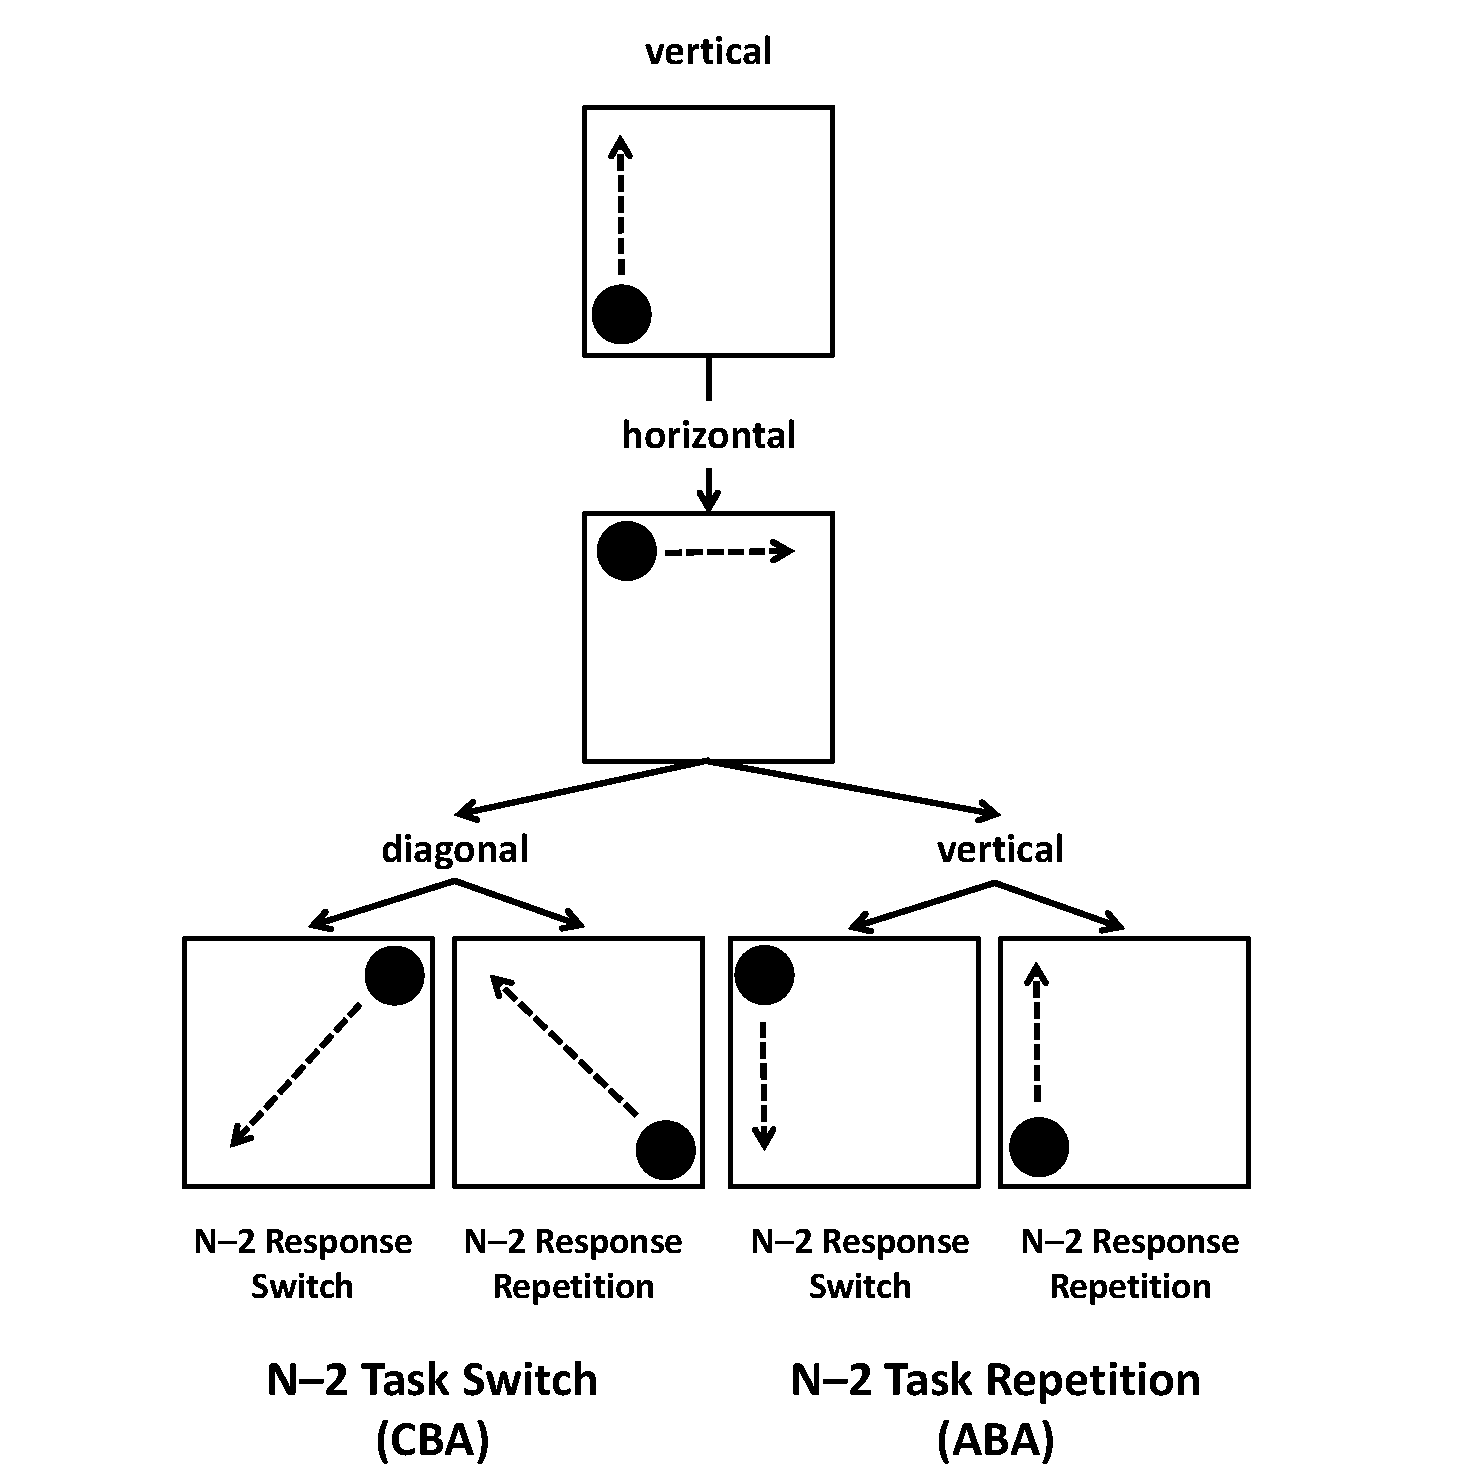
\includegraphics[width = \textwidth]{Images/mayrExperiment.pdf}
\caption{Schematic overview of Mayr's (2002) experimental procedure. The arrows are not displayed to participants, but reflect the spatial transformation required according to the given rule. See text for details.}
\label{fig:mayrExperiment}
\end{center}
\end{figure}


\cite{Mayr2002} found no statistically significant interaction between n--2 task repetition and n--2 response repetition [$F$(1, 38) = 1.3, $p$ = .26]; that is, there was no significant difference between n--2 task repetition costs for n--2 response repetitions and n--2 response switches. Mayr suggested this provided evidence against the episodic retrieval account of n--2 task repetition costs, and instead favours the inhibitory account.

\section{The Current Study}
The purpose of the current study was to re-examine the evidence for the effect of episodic retrieval on n--2 task repetition costs. The conclusion of \cite{Mayr2002} rests on the acceptance of a null hypothesis (i.e., no difference of n--2 task repetition costs), which cannot be achieved via standard null hypothesis significance testing \citep{Gallistel2009, Wagenmakers2007}; however, evidence in favour of a null hypothesis (given some data) can be obtained using Bayes factors \citep[e.g.,][]{Rouder2009}. The Bayes factor (denoted $BF_{10}$) quantifies the relative evidence provided by the data in favour of an alternative hypothesis (i.e., n--2 task repetition costs are different for response repetitions and response switches) over a null hypothesis (i.e., n--2 repetition costs are equivalent). 

The Bayes factor for the critical statistical test from Mayr's (2002) study ($BF_{10}$ = 0.315)\footnote{For all Bayes factors reported in this paper we use a non-informative prior on the alternative hypothesis, which is assumed to be distributed as a Cauchy with scaling factor $r$ = 0.707.} suggests that the null hypothesis is about 3 times more likely than the alternative, given the data, which provides anecdotal-to-moderate support for the null \citep[e.g.,][]{Schoenbrodtinpress}. As this Bayesian analysis does not provide compelling evidence for the null, and given the importance of assessing to what extent (if any) episodic retrieval can influence n--2 task repetition costs in task switching, we were interested in performing a replication of Mayr's study to gather more evidence.

The current study replicated critical aspects of Mayr's (2002) design relevant to n--2 task repetitions. As Mayr's study was also interested in exploring to what extent the rule-switching paradigm generated typical task switching effects (such as switch costs, effects of preparation, and effects of the delay between tasks), we made some changes to the original design so that it was more tailored toward assessing n--2 task repetition costs. Specifically, immediate task repetitions were not allowed; it has been shown that including immediate task repetitions reduces the n--2 task repetition cost \citep{Philipp2006}, so we removed this possibility. We also did not manipulate preparation via the cue--stimulus interval, as Mayr reported no effect of this variable on n--2 task repetition costs. Mayr did find that n--2 repetition costs were larger with shorter response--cue intervals (RCI; the time between the response to one trial and the onset of the cue for the next trial), a typical finding for n--2 task repetition costs \citep{Gade2005, Grange2009, Mayr2000}. Therefore, in order to obtain larger n--2 task repetition costs we only used a short RCI. 

%----------------------
\section{Method}

\subsection{Participants}
All participants were undergraduates at the School of Psychology at Keele University. Participants took part in exchange for partial course credit or a small cash payment (£6). Our final sample comprised 76 participants. Three additional participants were removed before analysis due to failure to maintain accuracy levels above 90\%.

Our sample size was determined via optional stopping. We used Sequential Bayes Factors \citep{Schoenbrodtinpress} to determine our stopping rule for participant recruitment. We were interested in establishing the presence or absence of an interaction between task sequence (ABA vs. CBA) and response repetition (repetition vs. switch). For the purposes of our stopping rule, this can be expressed as a default within-subjects Bayesian \emph{t}-test \citep{Rouder2009} comparing n--2 repetition costs for response repetitions and response switches.  We conducted a Bayesian \emph{t}-test on the data collected until the criterion for our a priori stopping rule was met. Specifically, our stopping rule required at least 20 participants; we continued data collection until $BF_{10}$ > 6 (constituting support for the alternative hypothesis) or $BF_{10}$ < 1/6 (constituting support for the null). \cite{Schoenbrodtinpress} demonstrated that a stopping rule of $BF_{10}$ > 6 (or $BF_{10}$ < 1/6) provided the best balance between type 1 and type 2 error, and was their recommended value for studies utilising Sequential Bayes Factors. 

\subsection{Apparatus \& Stimuli}
Stimuli were presented on a 17in. monitor connected to a PC running E-Prime v. 2.0 software. The stimulus display consisted of an 8cm by 8cm square frame. A black circle (diameter = 1 cm.) served as the trial stimulus. Possible cues were the words ``horizontal'', ``vertical'', or ``diagonal'', and were presented in size 22 black Verdanna font directly above the stimulus frame. Responses were collected via a 1-ms. precise USB keyboard.

\subsection{Procedure}
On each trial a cue was presented above the frame for 150ms. After this time, the circle stimulus appeared in one of the four corners of the frame. The cue remained on the screen during stimulus presentation. The task required participants to mentally make a spatial transformation of the stimulus' location according to the rule dictated by the task cue, and to make a spatially-congruent response to this translated location. For example, if the stimulus was in the top-right corner of the frame, the participant would need to make a top-left response if the task was ``horizontal'', a bottom-right response if the task was ``vertical'', and a bottom-left response if the task was ``diagonal''. Responses were made on the numerical part of the keyboard, using the ``4'', ``5'', ``1'', and ``2'' keys for top-left, top-right, bottom-left, and bottom-right responses respectively. Participants were asked to respond as quickly and as accurately as possible, using the index finger of their right hand. In between trials, participants were asked to place their finger in the centre of the four response keys. Once a response was registered, the frame was cleared for a response--cue interval of 150ms, after which time a new cue appeared for the next trial. The cue for the next trial was chosen randomly with the constraint that task repetitions could not occur (cf., Mayr, 2002); the stimulus location was chosen randomly with no constraints on each trial. If participants made an error, the word ``Error!'' appeared in red for 1000ms above the stimulus frame (in the cue's position).

Participants were presented with 16 trials as practice. The practice block was repeated once if the participant made more than four errors. The main experiment presented 4 blocks of 120 trials. 

\subsection{Design}
The experiment manipulated two factors in a fully-related design: \emph{Task Sequence} (n--2 task repetition [ABA] vs. n--2 task switch [CBA]) and \emph{Response Repetition} (n--2 response repetition vs. n-- response switch). The dependent variables were response time (RT) in milliseconds (ms.) and percent accuracy (\%).


%----------------------
\section{Results}
For response time analysis, the first two trials from each block were removed, as were error trials and the two trials following an error. Response times were trimmed by removing all RTs faster than 150ms, as well as any RTs slower than 2.5 standard deviations above the mean for each participant for each cell of the experimental design. Mean RTs and error rates can be seen in Table \ref{tab:behaviouralData}.

\begin{table*}[htbp]
\centering
\caption{Response times (RT) in milliseconds (ms) and accuracy (in percent) for ABA and CBA task sequences for response repetitions and response switches.}
\label{my-label}
\begin{tabular}{lccccc}
\hline
                    & \multicolumn{5}{c}{Task Sequence}                       \\ \cline{2-6} 
                    & \multicolumn{2}{c}{ABA}   &  & \multicolumn{2}{c}{CBA}  \\ \cline{2-3} \cline{5-6} 
                    & RT (ms)   & Accuracy (\%) &  & RT (ms)  & Accuracy (\%) \\ \hline
Response Repetition & 1000 (28) & 96.20 (0.39)  &  & 952 (28) & 96.36 (0.39) \\
Response Switch     & 1050 (29) & 95.02 (0.35)  &  & 964 (28) & 95.81 (0.34) \\ \hline
\end{tabular}
\label{tab:behaviouralData}
\end{table*}

\subsection{Response Times}
Response times were analysed via a two factor repeated measures analysis of variance (ANOVA) with the factors as described in \emph{Design}. There was a significant main effect of \emph{Sequence}, with slower RTs to ABA sequences (1,025ms) than to CBA sequences (958ms), $F$(1, 75) = 94.14, $p$<.001, $\eta_G^2$ = .018. The Bayes factor for this main effect was $BF_{10}$ = 1e+12, which provides substantial support for the presence of n--2 repetition costs. There was also a significant main effect of \emph{Response Sequence}, with faster RTs to response repetitions (976ms) than to response switches (1,007ms), $F$(1, 75) = 18.21, $p$<.001, $\eta_G^2$ = .004. The Bayes factor for this main effect was $BF_{10}$ = 338.77, which again provides substantial support for the alternative hypothesis. Critically, there was a significant interaction of both factors, $F$(1, 75) = 9.60, $p$<.01, $\eta_G^2$ = .001. The n--2 repetition cost was 48ms for response repetitions [$t$(75) = 4.2, $p$<.001; $BF_{10}$ = 271.24] and 86ms for response switches [$t$(75) = 13.0, $p$<.001; $BF_{10}$ = 7.11e+17]. 

The progression of the Sequential Bayes Factor for the interaction is shown in Figure \ref{fig:bayesFactor}. We stopped data collection after 76 participants, as at this point the criteria for our stopping rule had been reached\footnote{We could have stopped after 75 participants, but the last two participants were tested in successive sessions, so the Bayes factor was not checked until after the final participant.}. The final Bayes Factor for the difference of n--2 repetition costs for response repetitions and response switches was $BF_{10}$ = 9.97, which suggests that the alternative hypothesis is about 10 times more likely given than the data, which provides strong support that n--2 repetition costs are influenced by response repetitions.

\begin{figure*}
\begin{center}
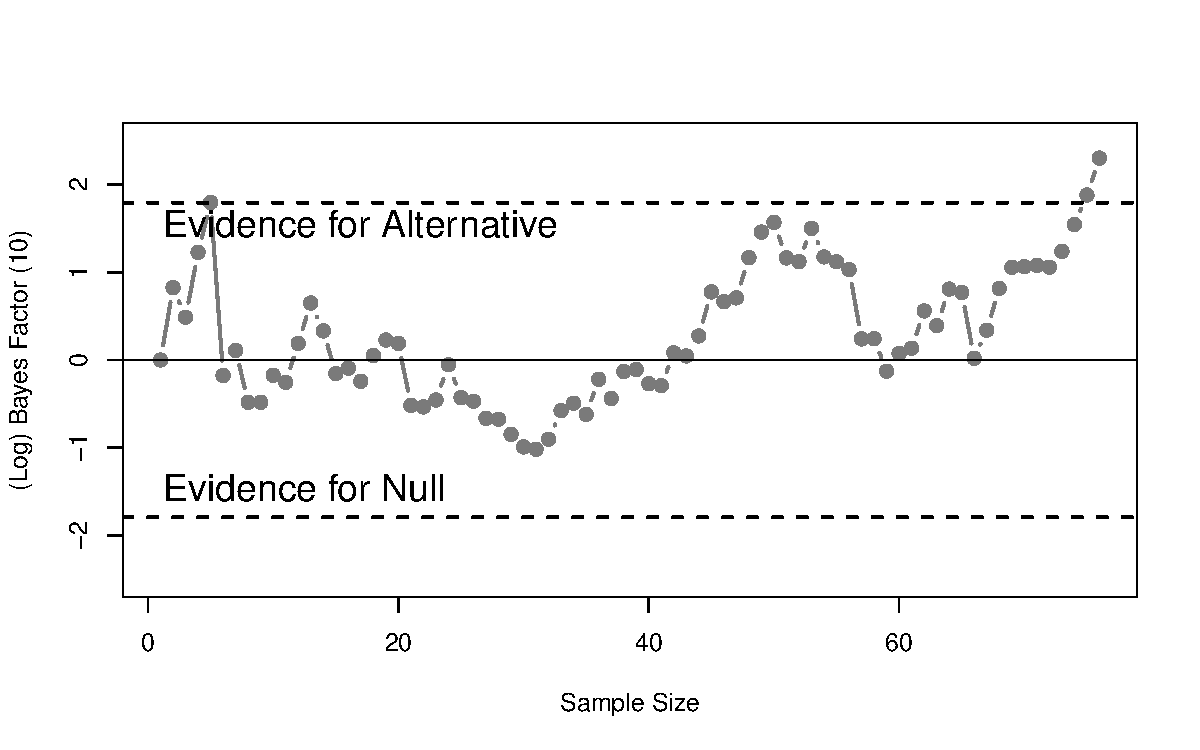
\includegraphics[width = \textwidth]{Images/bayesFactor.pdf}
\caption{Progression of the Sequential Bayes Factor [expressed as log($BF_{10}$)] as sample size increased. The criteria for a priori stopping rules are shown as dotted horizontal lines.}
\label{fig:bayesFactor}
\end{center}
\end{figure*}


\subsubsection{Robustness Check on Bayesian Priors}
We used a default prior distribution on the effect size for the alternative hypothesis in the Bayes factor analysis, which was assumed to be distributed as a Cauchy distribution with scale parameter $r$ = 0.707. To examine how robust our findings were to the choice of prior, we conducted a robustness check by re-calculating the Bayes factor across a wide range of priors by varying scale parameter $r$: As $r$ increases, the prior distribution becomes wider, reflecting a prior for larger effects; $r$s closer to zero make the distribution narrower, reflecting a prior for smaller effects. The robustness check is plotted in Figure \ref{fig:robustPrior}. This figure shows our conclusions (and our stopping rule) are robust to the prior used: Evidence favours the alternative hypothesis across all prior widths.

\begin{figure*}
\begin{center}
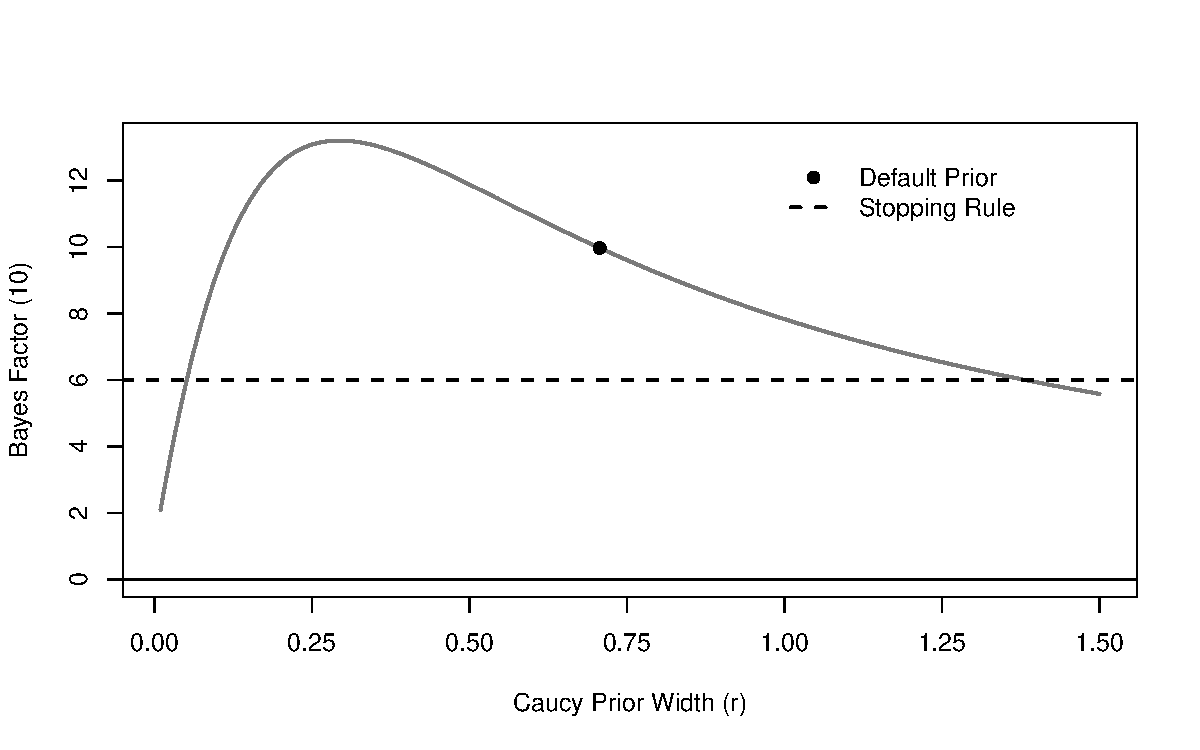
\includegraphics[width = \textwidth]{Images/robustPrior.pdf}
\caption{Robustness check of Bayes factor across a wide range of priors.}
\label{fig:robustPrior}
\end{center}
\end{figure*}


\subsubsection{Robustness of Recruitment Order on the Sequential Bayes Factor}
The progression of the Bayes Factor as sample size increased (Figure \ref{fig:bayesFactor}) appeared to provide slight evidence in favour of the null between sample sizes of 30 and 40, although the criterion for stopping was not reached. One might wonder, therefore, whether had a few more participants been recruited to the experiment showing a null interaction would we have stopped data collection and found evidence in favour of the null? Put another way, did recruitment order bias our results?

We wanted to assess how robust our stopping rule was to this apparent early evidence in favour of the null. Specifically, we were interested in whether our stopping rule in favour of the null would have been met had the participants been recruited in a different order. To assess this, we generated 50 random recruitment orders from our data set, and plotted the Sequential Bayes Factors for each recruitment order. If our findings are robust against recruitment order, the stopping rule in favour of the null should be rarely (if ever) met.  The results of this simulation are shown in Figure \ref{fig:recruitmentOrder}; each line represents the Sequential Bayes Factor for a random recruitment order. As can be seen, the stopping criterion in favour of the null is never met, suggesting our results are indeed robust to recruitment order. 

\begin{figure*}
\begin{center}
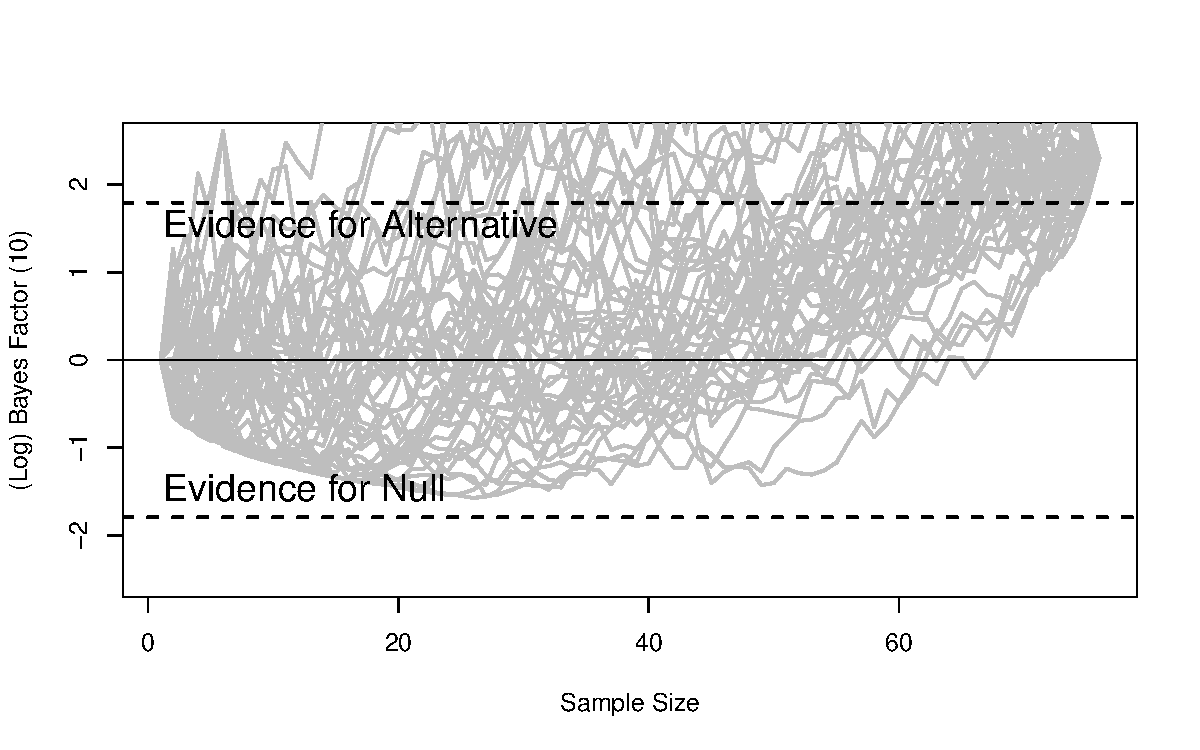
\includegraphics[width =  \textwidth]{Images/recruitmentOrder.pdf}
\caption{Simulated progression of the Sequential Bayes Factors for a random set of 50 different recruitment orders for the current data set. See text for details.}
\label{fig:recruitmentOrder}
\end{center}
\end{figure*}

\subsubsection{Bayesian Parameter Estimation}
We wished to supplement our Bayes factor analysis with Bayesian parameter estimation of the mean and effect size of the difference in n--2 task repetition cost between response repetitions and response switches. As such, we used the (default) methods outlined by \cite{Kruschke2013}. The input to the analysis was the n--2 task repetition cost for response repetitions minus the n--2 task repetition cost for response switches. The posterior distributions for mean difference and effect size of difference (Cohen's $d$) are shown in Figure \ref{fig:bayesParameter}.

\begin{figure*}
\begin{center}
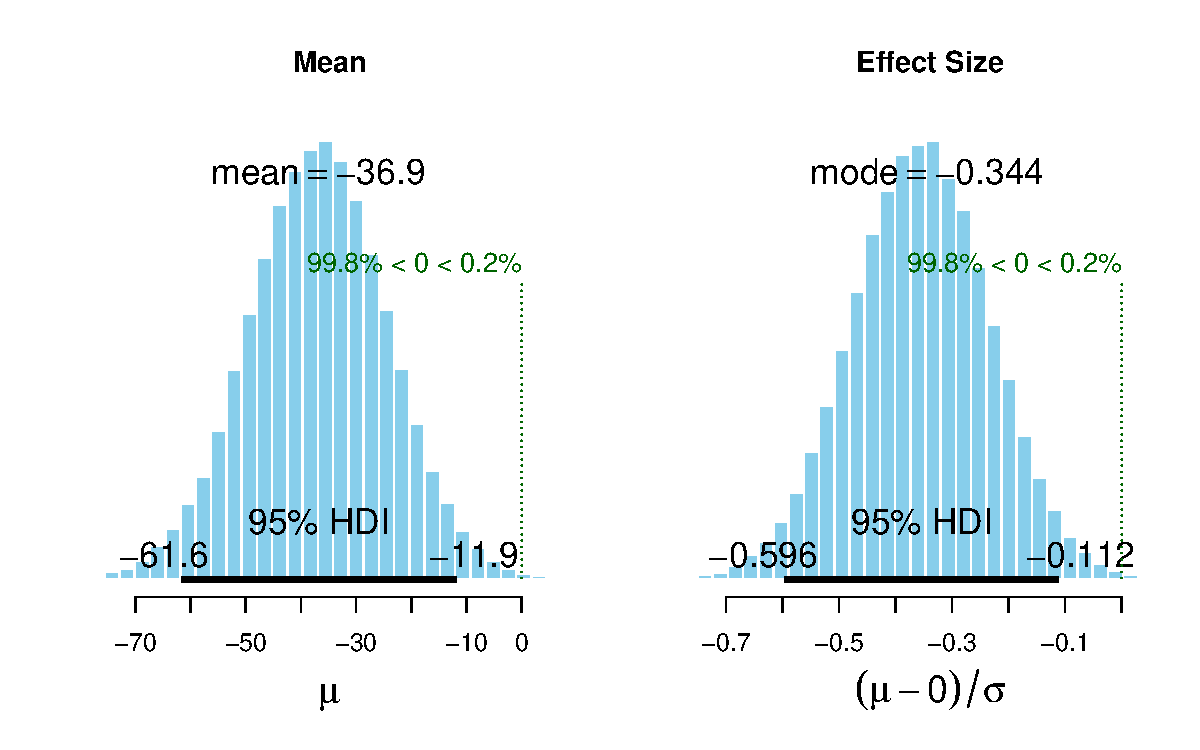
\includegraphics[width = \textwidth]{Images/bayesParameter.pdf}
\caption{Bayesian posterior distributions for the parameters of mean difference and effect size of difference for n--2 task repetition cost [response repetition] minus n--2 task repetition cost [response switch]. HDI = Highest Density Interval. See text for details.}
\label{fig:bayesParameter}
\end{center}
\end{figure*}

These posterior distributions present histograms of the Bayesian posterior estimate of the true mean and effect size underlying the data we obtained. The black horizontal bar represents the 95\% Highest Density Interval (HDI); in contrast to frequentist confidence intervals, we can interpret this interval as the range of parameter values we are 95\% certain the true underlying parameter lies within. The mean difference in n--2 task repetition costs for response repetitions and response switches is estimated to be -37ms; the HDI does not cross zero, so we can be confident that there is a difference between response repetitions and switches. Note, though, that the effect size of this difference is in the small range. For hypothesis testing (i.e., assessing whether episodic retrieval does impact the n--2 repetition cost or not), this is less relevant, but it is important to note if we wish to explore \emph{how much} episodic retrieval might affect n--2 repetition costs.

\subsection{Accuracy}
Accuracy analysis showed no significant effect of task sequence [$F$(1, 75) = 3.36, $p$=.07, $\eta_G^2$ = .006]; the Bayes factor for this main effect was $BF_{10}$ = 0.618, which provides only anecdotal support for the null. The main effect of response repetition was significant [$F$(1, 75) = 12.17, $p$<.001, $\eta_G^2$ = .019], suggestive of better accuracy for response repetitions (96.28\%) than for response switches (95.41\%). The Bayes factor was $BF_{10}$ = 29.66, which provides strong support for the alternative. The interaction was not significant [$F$(1, 75) = 1.32, $p$=.25, $\eta_G^2$ = .003]; the Bayes factor was $BF_{10}$ = 0.238, which provides moderate support for the null hypothesis.

%----------------------
\section{Discussion}

The present study sought to re-examine the evidence for any potential effect of episodic retrieval on n--2 task repetition costs in task switching by replicating key aspects of Mayr's (2002) study. In contrast to that study, we found clear evidence of episodic retrieval influencing n--2 task repetition costs in task switching; specifically, n--2 task repetition costs were smaller when the response repeated over an ABA sequence compared to when the response switched. This is in line with an episodic retrieval account which produces facilitation to responding when trial parameters match over an ABA sequence (i.e., for n--2 response repetitions). This facilitation to performance can reduce to some extent the n--2 task repetition cost, suggesting episodic retrieval can reduce the negative effects of inhibition when trial parameters match.

This finding has important implications for theories of task switching. There is growing evidence that episodic retrieval plays a role in explaining several task switching effects. For example, \cite{Altmann2011} provided empirical and theoretical evidence that episodic retrieval can explain the response-repetition effect in task switching, the observation that task repetition RTs are facilitated when the required response repeats from trial n--1 to the current trial, yet response repetitions produce a cost for task switches. \cite{Horoufchin2011a} \citep[see also][]{Horoufchin2011} also provided evidence that episodic retrieval can explain some task switching effects. It is typically found that the switch cost is reduced at longer RCIs \cite[e.g.,][]{Meiran2000a}; the standard explanation for this finding pertains to the decay of task representations in memory reducing task repetition RTs. However, \cite{Horoufchin2011a} provided compelling evidence that this pattern of data can be better explained with reference to episodic retrieval account: trialwise variation of the RCI affects the \emph{temporal distinctiveness} of task traces in episodic memory, thus influencing their retrieval probability \citep{Brown2007,Grange2015}. The current work extends this evidence of the role of episodic retrieval influencing task switching effects. As such, theoretical accounts of cognitive control during task switching will have to take into account the role of episodic retrieval. 

For clarification, note that we have not provided evidence that episodic retrieval can explain the n--2 task repetition cost entirely, but rather that it reduces the cost. Indeed, the n--2 task repetition cost was still statistically significant even when the trial parameters matched across n--2 task repetitions (i.e., n--2 response repetitions). Therefore, our findings do not provide evidence against the inhibitory explanation of these costs. Rather, we have shown that these costs can be reduced with successful episodic retrieval. As such, researchers should be cognisant of the potential contribution of episodic retrieval mismatches inflating estimates of n--2 task repetition costs when wishing to use this effect for measuring inhibition.

Our results differ to those reported by \cite{Mayr2002}. We suggest that our modifications to Mayr's original design improved the sensitivity of the paradigm to be able to detect potential episodic retrieval effects on n--2 task repetitions. The modifications were made to enhance the magnitude of n--2 task repetition costs, so that modulation of this cost with response repetitions could be more easily detected. Specifically, removing the possibility of immediate task repetitions likely enhanced the n--2 task repetition cost as it has been shown that allowing immediate repetitions reduces this cost \citep{Philipp2006}. We also used the shortest RCI used by Mayr (150ms), as it is a consistent finding that this increases the n--2 repetition cost \cite{Gade2005, Grange2009, Mayr2000, Mayr2002}. Any one of these modifications could explain the difference in results between this study and that of Mayr (2002). Future research should aim to examine the potential role for episodic retrieval influencing n--2 task repetition costs by providing further replications and conceptual extensions to this study \citep{OpenScienceCollaboration2015}.



%%%--------------------------------------------------------------------------------------------


%%%--------------------------------------------------------------------------------------------
\bibliography{References.bib}

\end{document}
